\documentclass{article}
\usepackage[utf8]{inputenc}
\usepackage{amssymb}
\usepackage{graphicx}
\usepackage{setspace}
\usepackage{listings}
\usepackage{float}
\usepackage{xcolor}
\usepackage{amsmath}
\usepackage{pgfplots}
\usepackage{enumitem}
\usepackage{subcaption}

\title{\textbf{High Performance Computer Architectures Practical Course \\ - Exercise 2 -} \\[10mm]}
\author{Tutorium 1 \\[10mm] David Jordan (6260776) \\[1mm] Florian Rüffer (7454628) \\[1mm] Michael Samjatin (7485765) \\[10mm]}


\lstset{
    language=C++,
    basicstyle=\ttfamily,
    keywordstyle=\color{blue},
    stringstyle=\color{red},
    commentstyle=\color{green},
    numbers=left,
    numberstyle=\normalsize,
    breaklines=true,
    showstringspaces=false,
    frame=single,
    linewidth=1\linewidth,
    captionpos=b
}


\begin{document}
\maketitle
\newpage
\section*{Problem 1}
% To add numbered subsection / section / etc. remove "*".
\subsection*{Add subsection}
\subsection*{Add subsection}
\subsection*{Add subsection}
\section*{Problem 2}
% To add numbered subsection / section / etc. remove "*".
\subsection{Add subsection}
\subsection{Add subsection}
\subsection{Add subsection}
\renewcommand{\lstlistingname}{File}% Listing -> Algorithm
\renewcommand{\lstlistlistingname}{List of \lstlistingname s}% List of Listings -> List of Algorithms

\begin{lstlisting}[caption=Add caption]
std::vector<float> MLPMath::applyReLU(std::vector<float>& input) {

    std::vector<float> result(input.size());

    for (std::size_t i = 0; i < input.size(); i++) {

        if (input[i] >= 0) {  
            result[i] = input[i];
        }
        else {
            result[i] = 0.0f;
        }
    }

    return result;
}
\end{lstlisting}

\begin{center}

\begin{tikzpicture}
\begin{axis}[
    xlabel={$x$},
    ylabel={$y$},
    axis lines=middle,
    xmin=-5, xmax=5,
    ymin=-0.5, ymax=5,
    xtick={-5,-4,-3,-2,-1,0,1,2,3,4,5},
    ytick={0,1,2,3,4,5},
    yticklabels={0,1,2,3,4,5},
    xticklabels={-5,-4,-3,-2,-1,0,1,2,3,4,5},
    samples=100,
    domain=-5:5,
    smooth,
    thick
]
\addplot+[mark=none] {max(0,x)};
\end{axis}
\end{tikzpicture}
\end{center}
\[
\text{ReLU}(x) =
\begin{cases}
x, & \text{if } x \geq 0 \\
0, & \text{otherwise}
\end{cases}
\]



\begin{figure}[H]
  \centering
  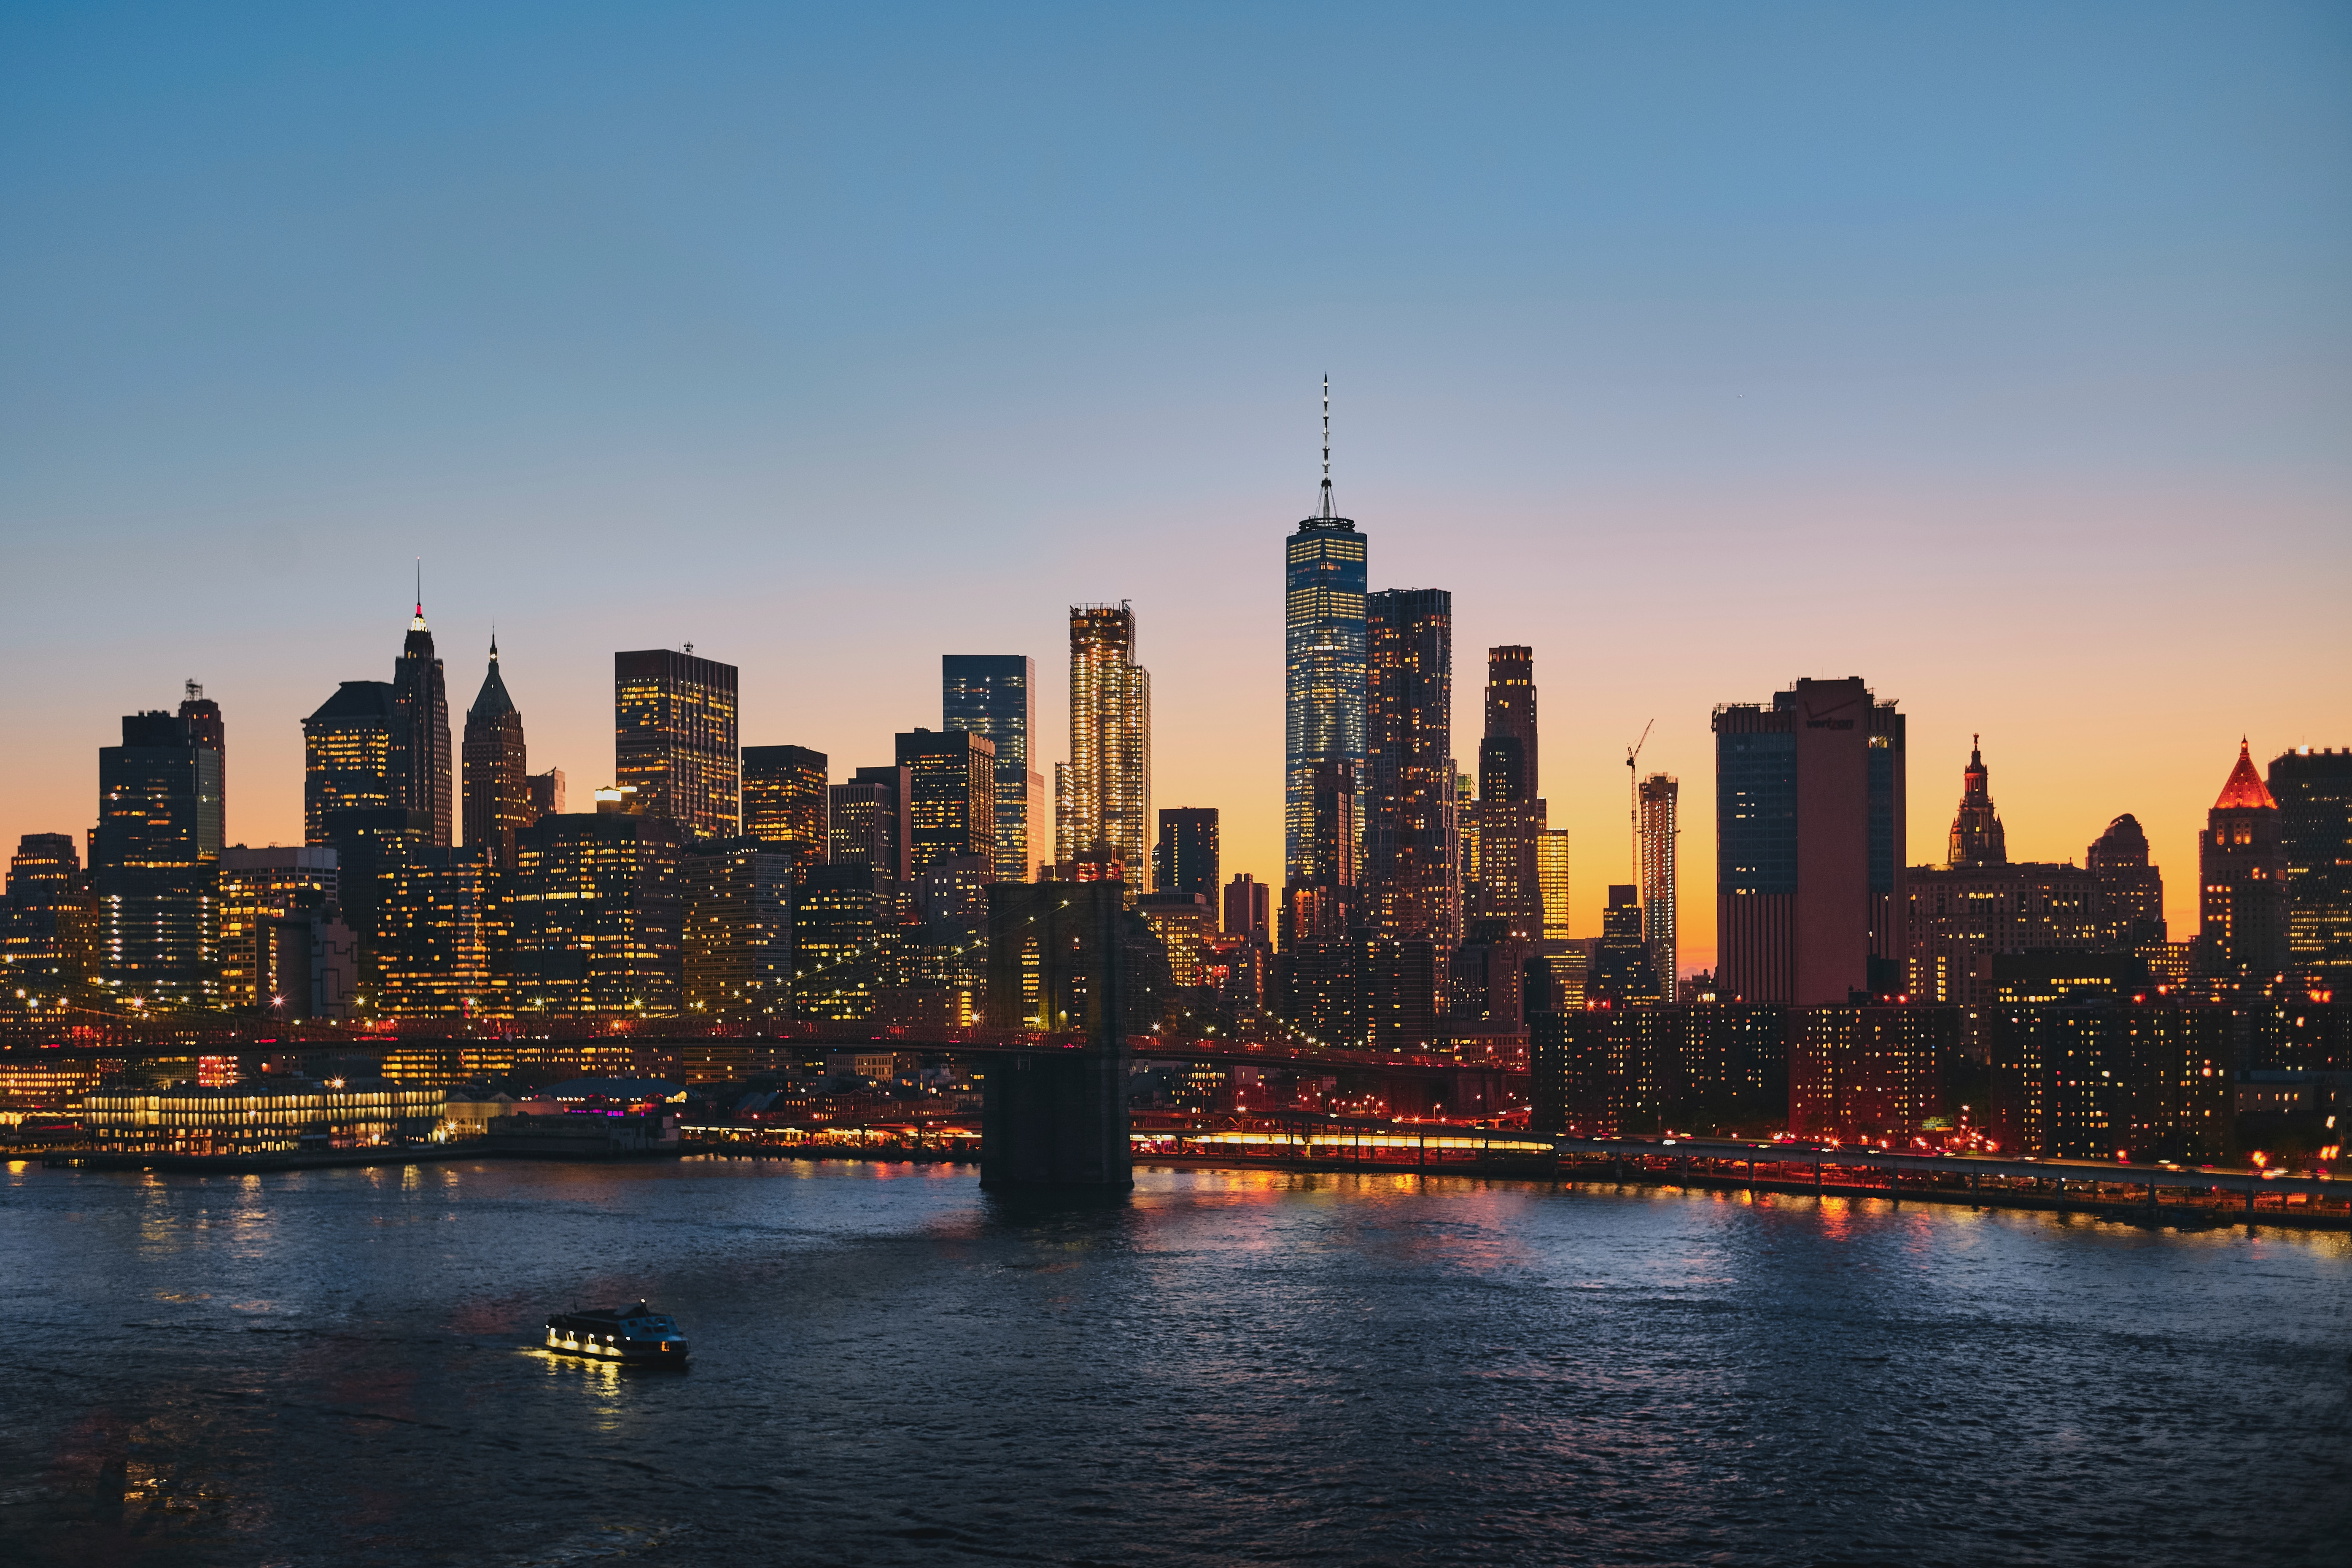
\includegraphics[width=\textwidth]{filler.png} 
  \caption{Add caption}
  \label{fig:example}
\end{figure}


\end{document}
